%%%%%%%%%%%%%%%%%%%%%%%%%%%%%%%%%%%%%%%%%
% Short Sectioned Assignment LaTeX Template Version 1.0 (5/5/12)
% This template has been downloaded from: http://www.LaTeXTemplates.com
% Original author:  Frits Wenneker (http://www.howtotex.com)
% License: CC BY-NC-SA 3.0 (http://creativecommons.org/licenses/by-nc-sa/3.0/)
%%%%%%%%%%%%%%%%%%%%%%%%%%%%%%%%%%%%%%%%%

% \documentclass[paper=a4, fontsize=11pt]{scrartcl} % A4 paper and 11pt font size
\documentclass[11pt, a4paper]{book}
\usepackage[T1]{fontenc} % Use 8-bit encoding that has 256 glyphs
\usepackage[utf8]{inputenc}
\usepackage{fourier} % Use the Adobe Utopia font for the document - comment this line to return to the LaTeX default
\usepackage{listings} % para insertar código con formato similar al editor
\usepackage[spanish]{babel} % Selecciona el español para palabras introducidas automáticamente, p.ej. "septiembre" en la fecha y especifica que se use la palabra Tabla en vez de Cuadro
\usepackage{url} % ,href} %para incluir URLs e hipervínculos dentro del texto (aunque hay que instalar href)
\usepackage{graphics,graphicx, float} %para incluir imágenes y colocarlas
\usepackage[gen]{eurosym} %para incluir el símbolo del euro
\usepackage{cite} %para incluir citas del archivo <nombre>.bib
\usepackage{enumerate}
\usepackage{hyperref}
\usepackage{graphicx}
\usepackage{tabularx}
\usepackage{booktabs}

\usepackage[table,xcdraw]{xcolor}
\hypersetup{
	colorlinks=true,	% false: boxed links; true: colored links
	linkcolor=black,	% color of internal links
	urlcolor=cyan		% color of external links
}
\renewcommand{\familydefault}{\sfdefault}
\usepackage{fancyhdr} % Custom headers and footers
\pagestyle{fancyplain} % Makes all pages in the document conform to the custom headers and footers
\fancyhead[L]{} % Empty left header
\fancyhead[C]{} % Empty center header
\fancyhead[R]{José Miguel Pelegrina Pelegrina} % My name
\fancyfoot[L]{} % Empty left footer
\fancyfoot[C]{} % Empty center footer
\fancyfoot[R]{\thepage} % Page numbering for right footer
%\renewcommand{\headrulewidth}{0pt} % Remove header underlines
\renewcommand{\footrulewidth}{0pt} % Remove footer underlines
\setlength{\headheight}{13.6pt} % Customize the height of the header

\usepackage{titlesec, blindtext, color}
\definecolor{gray75}{gray}{0.75}
\newcommand{\hsp}{\hspace{20pt}}
\titleformat{\chapter}[hang]{\Huge\bfseries}{\thechapter\hsp\textcolor{gray75}{|}\hsp}{0pt}{\Huge\bfseries}
\setcounter{secnumdepth}{4}
\usepackage[Lenny]{fncychap}
\graphicspath{ {./imagenes/} } 

\begin{document}

	% Plantilla portada UGR
	\begin{titlepage}
\newlength{\centeroffset}
\setlength{\centeroffset}{-0.5\oddsidemargin}
\addtolength{\centeroffset}{0.5\evensidemargin}
\thispagestyle{empty}

\noindent\hspace*{\centeroffset}\begin{minipage}{\textwidth}

\centering

\includegraphics[width=0.9\textwidth]{logos/logo_ugr.jpg}\\[1.4cm]

\textsc{ \Large TRABAJO FIN DE GRADO\\[0.2cm]}
\textsc{ GRADO EN INGENIERIA INFORMATICA}\\[1cm]

{\Huge\bfseries Generación de dietas optimizadas con fines concretos \\}
\noindent\rule[-1ex]{\textwidth}{3pt}\\[3.5ex]
% {\large\bfseries Subtítulo }
\end{minipage}

\vspace{1.5cm}
\noindent\hspace*{\centeroffset}
\begin{minipage}{\textwidth}
\centering

\textbf{Autor}\\ {José Miguel Pelegrina Pelegrina}\\[2.5ex]
\textbf{Director}\\ {Juan Julián Merelo Guervós)}\\[2cm]

\includegraphics[width=0.3\textwidth]{logos/etsiit_logo.png}\\[0.1cm]
\textsc{Escuela Técnica Superior de Ingenierías Informática y de Telecomunicación}\\
\textsc{---}\\
Granada, Junio de 2021
\end{minipage}
\end{titlepage}


	% Plantilla prefacio UGR
	\thispagestyle{empty}

\begin{center}
{\large\bfseries OrganizeUDiet \\ Generación de dietas optimizadas con fines concretos}\\
\end{center}
\begin{center}
José Miguel Pelegrina Pelegrina\\
\end{center}

%\vspace{0.7cm}

\vspace{0.5cm}
\noindent{\textbf{Palabras clave}: \textit{Python, Django, Nutrición, Dieta, Software libre}\\
\vspace{0.7cm}
\noindent{\textbf{Resumen}
\cleardoublepage

\begin{center}
	{\large\bfseries OrganizeUDiet \\ Generation of optimized diets for specific purposes}\\
\end{center}
\begin{center}
	José Miguel Pelegrina Pelegrina\\
\end{center}
\vspace{0.5cm}
\noindent{\textbf{Keywords}: \textit{Python, Django, Nutrition, Diet, Open source}
\vspace{0.7cm}

\noindent{\textbf{Abstract}

\cleardoublepage

\thispagestyle{empty}

\noindent\rule[-1ex]{\textwidth}{2pt}\\[4.5ex]

D. \textbf{Juan Julián Merelo Guervós}, Profesor del Departamento de Arquitectura y Tecnología de Computadores de la Universidad de Granada.

\vspace{0.5cm}

\textbf{Informo:}

\vspace{0.5cm}

Que el presente trabajo, titulado \textit{\textbf{Generación de dietas optimizadas con fines concretos}},
ha sido realizado bajo mi supervisión por \textbf{José Miguel Pelegrina Pelegrina}, y autorizo la defensa de dicho trabajo ante el tribunal
que corresponda.

\vspace{0.5cm}

Y para que conste, expiden y firman el presente informe en Granada a Junio de 2021.

\vspace{1cm}

\textbf{El/la director(a)/es: }

\vspace{5cm}

\noindent \textbf{Juan Julián Merelo Guervós}

\chapter*{Agradecimientos}






	% Índice de contenidos
	\newpage
	\tableofcontents

	% Índice de imágenes y tablas
	\newpage
	\listoffigures

	% Si hay suficientes se incluirá dicho índice
	\listoftables 
	\newpage

	% Introducción 
	\chapter{Introducción}

Este proyecto es software libre, y está liberado con la licencia \cite{gplv3}.
\\\\
Ante la situación actual que vivimos con el covid-19, muchas personas han decidido 
hacer deporte para así mantenerse en forma debido a los confinamientos
o el teletrabajo o simplemente para despejarse de la situación y no estar aislados en casa. 
Además muchas personas quieren acompañar este deporte con una dieta o simplemente quieren hacer 
dieta para mantenerse saludables.
\\\\
Para ello estamos obligados a tener un dietista contratado todos los meses y tener recursos para 
comprar los productos que nos mandan y muchas personas o no tienen recursos o simplemente preferirían
que hubiera una aplicación en la que ellos mismos pudieran obtener su dieta y modificarla según sus 
posibilidades o gustos.
\\\\

\section{Descripción del problema}

Este proyecto es facilitar a las personas la obtención de una dieta sin tener que 
contratar un dietista y poder modificarla en base a sus gustos o posibilidades.
\\\\
Actualmente con la situación que estamos viviendo muchas personas, en las que me incluyo, hemos 
decidido practicar algún deporte o simplemente hacer ejercicio además de acompañarlo con una dieta 
para mantenernos saludables y en forma, ya que con el teletrabajo, clases online y confinamiento.
\\\\
En mi caso y en el de muchas personas hemos tenido que contratar un dietista que nos lleve la dieta 
cada mes además de tener que comprar productos que o no podemos permitirnos o no tenemos en casa y no 
podemos/queremos ir a comprarlos o simplemente no nos gustan.
\\\\
El objetivo de este proyecto es facilitar la obtención de una dieta a todas las personas haciendolo mucho 
mas cómodo consultando una web que contratando y estando en contacto con un dietista además de dar la posibilidad 
de recomendar productos similares.




	% Descripción del problema
	\chapter{Descripción del problema}

Este proyecto es facilitar a las personas la obtención de una dieta sin tener que 
contratar un dietista y poder modificarla en base a sus gustos o posibilidades.
\\\\
Actualmente con la situación que estamos viviendo muchas personas, en las que me incluyo, hemos 
decidido practicar algún deporte o simplemente hacer ejercicio además de acompañarlo con una dieta 
para mantenernos saludables y en forma, ya que con el teletrabajo, clases online y confinamiento.
\\\\
En mi caso y en el de muchas personas hemos tenido que contratar un dietista que nos lleve la dieta 
cada mes además de tener que comprar productos que o no podemos permitirnos o no tenemos en casa y no 
podemos/queremos ir a comprarlos o simplemente no nos gustan.
\\\\
El objetivo de este proyecto es facilitar la obtención de una dieta a todas las personas haciendolo mucho 
mas cómodo consultando una web que contratando y estando en contacto con un dietista además de dar la posibilidad 
de recomendar productos similares.

	% Estado del arte
	\chapter{Estado del arte}

El software libre y sus licencias \cite{gplv3} ha permitido llevar a cabo una expansión del
aprendizaje de la informática sin precedentes.

En este apartado lo que pretende es mostrar como se encuentra el panorama en el cual vamos a llevar a cabo nuestro proyecto. Para ello, en primer lugar realizaremos un análisis del mercado, donde se presentarán las principales alternativas a nuestra idea de proyecto ya existentes, de forma que analicemos los requisitos de nuestro sistema comparándolo con los de aquellos que ya existen. En segundo lugar analizaremos punto por punto los recursos utilizados para poder llevar a cabo este proyecto.

\section{Análisis de mercado}

En el Capítulo~\ref{ch:introduccion} comentábamos que el acceso a los datos ya era algo posible para toda la población. Esto se debe a que son de dominio público y es el propio gobierno de España o las Comunidades Autónomas los que publican los datos en sus respectivas web. Dado que este proyecto está centrado en la visualización de datos, es muy importante poder realizar una comparación de los requisitos que queremos presentar en el mismo con las diversas funcionalidades de otras aplicaciones englobadas dentro del mismo género. Por desgracia, tras realizar una búsqueda de aplicaciones en la \textbf{Play Store} de Google a fecha de Noviembre de 2020, el resultado mostrado a sido bastante sorprendente. Según \textbf{Play Store}, no hay ningún tipo de aplicación similar a lo que se pretende desarrollar en este proyecto. Ejemplo de ello son las aplicaciones que nos sugiere:

\begin{itemize}
	\item \textbf{Radar COVID:} Aplicación de alertas en caso de haber estado cerca de alguien que tiene COVID-19
	\item \textbf{GVA Coronavirus:} Aplicación de la Generalitat Valenciana para solicitar citas en caso de mostrar síntomas.
	\item \textbf{PassCOVIS.gal} Aplicación de la Xunta de Galicia para recibir avisos, información de las restricciones, recomendaciones y novedades.
	\item \textbf{COVIS-19.eus} Aplicación del Gobierno del País Vasco para realizar un auto-diagnóstico y avisar a tu círculo de personas.
	\item \textbf{CONFINAPP} Aplicación que pretende ser un acompañamiento y la puerta de entrada a la información y servicios de la Generalitat de Cataluña.
\end{itemize}

Visto que en el ámbito de las aplicaciones móviles no encontramos nada similar, tendremos que hacer una comparación con la principal fuente actual de información de la que disponemos, el \textbf{Gobierno de España}.

En este punto, antes que hacer el análisis, debemos conocer cuales son los requisitos que queremos tener en nuestra aplicación. Tras un estudio de los datos, siguiendo un criterio propio, he recogido las funcionalidades principales con las que debería contar una aplicación como la que se va a desarrollar y que permitan al propio usuario tener acceso a la misma sin ningún conocimiento previo. Estas funcionalidades por consiguiente sí están presentes en \textbf{Covid-19 Reports} y son las siguientes:

\begin{enumerate}
	\item Seleccionar la Comunidad Autónoma sobre la que se quieren conocer los datos.
	\item Visualización del incremento de casos, casos acumulados, media de la última semana y últimas 24h.
	\item Visualización de los fallecimientos acumulados, media de la última semana y últimas 24 horas.
	\item Visualización de los datos de hospitalización, camas y camas UCI ocupadas, porcentaje del total de camas, altas e ingresos.
	\item Visualización de casos y muertes según la edad, solo al consultar datos de España.
	\item Visualización de los casos por cada 100mil habitantes, solo al consultar datos de España.
	\item Visualización de los casos por cada 100mil habitantes en la última semana, solo al consultar datos de España.
	\item Visualización de los fallecidos por cada 100mil habitantes, solo al consultar datos de España.
	\item Visualización de los fallecidos por cada 100mil habitantes en la última semana, solo al consultar datos de España.
	\item Visualización ordenada y clara.
	\item Toda la información es gratuita.
	\item No tiene ampliaciones de pago.
	\item No tiene anuncios.
	\item Plataforma móvil donde se ofrece
\end{enumerate}

\subsection{Representación de datos Covid-19 en España}

Como hemos dicho antes, llevaremos a cabo un análisis de como se representan los datos por parte del \textbf{Gobierno de España}. Para ello tendremos que acceder a la página web de \textbf{Gobierno de España}, donde podemos consultar los datos del conjunto del territorio español. Teniendo en cuenta que no se trata de una aplicación si no de una web, se ha creído conveniente que los puntos 11-14 no es necesario analizarlos.

A primera vista el acceso a la información desde el navegador aparenta ser sencillo. El usuario tiene que acceder a la web de La Moncloa \cite{la-moncloa}, desde ahí se accederá a una pequeña pestaña llamada \textit{Covid-19}, la cual mostrará una serie de opciones, como se puede ver en la Figura \ref{fig:inicio-moncloa} y cuya opción a seleccionar será \textit{Cifras de la situación}.

\begin{figure}[H]
	\centering
	\includegraphics[width=1\textwidth]{img/inicio-moncloa}
	\caption{Página de inicio La Moncloa.}
	\label{fig:inicio-moncloa}
\end{figure}

\newpage
Una vez se ha redirigido al usuario, se le dará la opción de consultar los datos de España o los datos globales, junto con la opción de visualizar un video del proceso de recogida los datos en España, como se muestra en la Figura \ref{fig:opciones-moncloa}. Para este caso, la opción sobre la que nos centraremos es concretamente la que nos permite acceder a los datos a nivel de España, el usuario la seleccionará y será redirigido a una web del Ministerio de Sanidad \cite{gob-espana}, la cual vemos en la Figura \ref{fig:ministerio-salud}.

\begin{figure}[H]
	\centering
	\includegraphics[width=1\textwidth]{img/opciones-moncloa}
	\caption{Opciones de consulta de La Moncloa.}
	\label{fig:opciones-moncloa}
\end{figure}

\begin{figure}[H]
	\centering
	\includegraphics[width=1\textwidth]{img/ministerio-salud}
	\caption{Página de consulta del Covid-19 del Ministerio de Sanidad.}
	\label{fig:ministerio-salud}
\end{figure}

Dentro de la página del Ministerio de Sanidad lo primero que llama la atención y más resalta es el total de casos confirmados a nivel de España, de Europa y del Mundo. Además se indica al usuario que los datos, debido a la situación excepcional, se publicarán los lunes, de manera que la evolución de estos se verá semanalmente. Dentro de las opciones que se permiten seleccionar, el usuario tendrá seleccionar dos de ellas, en primer lugar \textit{Situación de COVID-19 en España}, la cual redirigirá al usuario a un mapa del territorio español interactivo donde lo único que se podrá consultar será la incidencia acumulada de las Comunidades Autónomas en los últimos 7 y 14 días como se muestra en la Figura \ref{fig:mapa-situacion}.

\begin{figure}[H]
	\centering
	\includegraphics[width=1\textwidth]{img/mapa-situación}
	\caption{Mapa con la incidencia acumulada por Comunidades Autónomas.}
	\label{fig:mapa-situacion}
\end{figure}

Otras de las opciones que el usuario puede seleccionar es la \textit{Actualización nº X}, que le permitirá visionar un pdf donde se encuentra toda la información unificada en tablas y posteriormente una serie de gráficas asociadas a las mismas. Dentro de toda la información que se nos proporciona, podemos ver la siguiente repartida en diversas tablas:

\begin{itemize}
	\item Casos de COVID-19 confirmados totales, diagnosticados el día previo y diagnosticados o con fecha de inicio de síntomas en los últimos 14 y 7 días.
	\item Casos de COVID-19 que han precisado hospitalización e ingreso en UCI.
	\item Situación capacidad asistencial y actividad Covid-19 en hospitales.
	\item Total de Pruebas diagnósticas realizadas.
	\item Casos de COVID-19 que han fallecido (total y con fecha de fallecimiento en los últimos 7 días).
	\item Nº de casos COVID-19 importados de otro país.
	\item Detalles de los quince países con más casos confirmados de Europa
	\item Casos confirmados de COVID-19 fuera de Europa.
	\item Detalles de los quince países con más casos confirmados fuera de Europa
\end{itemize}

Si se quiere ver el modelo con el que se muestra esta información podemos acceder desde aquí \cite{actualizacion-gob}.

Como se ha podido de ver en el análisis, el acceso a los datos que nos proporciona el \textbf{Gobierno de España} es más o menos sencillo, pero para la gente que apenas usa esta web, mostrar un archivo pdf donde se representen enormes tablas con diversos datos que, aunque relacionados, cuando superan cierta cantidad pueden llegar a ser confusos, y gráficas separadas por varias páginas de estas tablas de datos, no es la mejor práctica posible.

\subsection{Comparativa}

Una vez hecho el análisis de la única opción conocida que puede llegar a aportar datos similares a los que queremos mostrar con nuestra aplicación, procederemos a hacer una comparativa con los diferentes requisitos que definimos con anterioridad.

Como hemos dicho antes, no compararemos los puntos 11-14 porque estos se han considerado que están asociados a un aplicación móvil y no a una página web como es el caso. En cuanto a los requisitos restantes, en referencia al 1, es cierto que podemos ver los datos de las diferentes Comunidades Autónomas, pero al tratarse de un simple documento pdf es imposible realizar una selección de las mismas.

En cuanto al resto de requisitos (2-9), todos ellos son visibles dentro del documento que nos proporciona la página web. En cuanto al requisito 10, queda claro, como se ha mencionado antes, que la visualización tanto de datos y gráficas no es ordenada y mucho menos clara, sobre todo cuando se acumulan varios tipos de información.

Es cierto que en la información proporcionada por el \textbf{Gobierno de España} es muy completa, como debe esperarse de la máxima autoridad del país, pero eso no hace que sea perfecta. La principal idea de la aplicación que se va a desarrollar es poder facilitar el acceso a estos datos al usuario, permitiéndole acceder de manera sencilla e intuitiva a los mismos y seleccionar la información que desea utilizar. Es decir, lo que se pretende es una aplicación sencilla e interactiva, cosa que no se nos proporciona por parte del \textbf{Gobierno de España}.

\section{Recursos necesarios} \label{sec:recursos}

\subsection{Telegram}

\begin{figure}[H]
	\centering
	\includegraphics[width=0.2\textwidth]{img/telegram-icon}
	\caption{Logotipo de Telegram.}
\end{figure}

\textbf{Covid-19 Reports} está concebido para ser un chatbot, por lo que la primera decisión que se ha tenido que tomar ha sido la plataforma donde se implementará. Hay muchas aplicaciones sobres las que se podría llevar a cabo el desarrollo de este chatbot, aunque para este punto se han considerado solo dos de ellas: WhatsApp \cite{whatsapp} y Telegram \cite{telegram}. En un artículo de la web Xataka Android \cite{articulo-xataka}, se lleva a cabo una explicación punto por punto de las diferencias entre ambas aplicaciones finalizando con una tabla que mostramos en la Figura \ref{fig:tabla-comparativa}

\begin{figure}[H]
	\centering
	\includegraphics[width=0.6\textwidth]{img/tabla-comparativa}
	\caption{Tabla comparativa WhatsApp vs Telegram. Fuente: Xataka \cite{articulo-xataka}}
	\label{fig:tabla-comparativa}
\end{figure}

Existen varias razones por las que se ha optado por hacer uso de \textbf{Telegram}, entre ellas podemos destacar las siguientes:

\begin{enumerate}
	\item \textbf{Contenido disponible a través de Bots:} en el caso de \textbf{Telegram}, la lista de contenidos se ve multiplicada gracias a estos. Es cierto que \textbf{WhatsApp} también puede permitir la implementación de Bots, pero aún no es algo que se pueda realizar de manera generalizada, mientras que en \textbf{Telegram} cualquier usuario puede crear sus propios Bots.
	\item \textbf{Cuentas asociadas a un nº de teléfono:} \textbf{WhatsApp} tiene sus cuentas de usuario enlazadas a los números de teléfono de los usuarios, lo que implica que no se puede chatear con alguien sin tener su nº de teléfono. Sin embargo, \textbf{Telegram} facilita la comunicación entre usuarios asignándole nombres de usuarios a los mismos. Esto implica un importante punto a favor de \textbf{Telegram} en el ámbito de la privacidad, ya que en \textbf{WhatsApp} mientras formemos parte de un grupo todos los usuarios que se encuentre en este pueden ver nuestro nº de teléfono, \textbf{Telegram} mostrará en su lugar el nombre de usuario, impidiendo al resto conocer nuestro nº de teléfono.
	\item \textbf{Versión Web:} En este punto \textbf{Telegram} es el claro ganador. Aunque las dos aplicaciones cuentan con una versión Web, \textbf{WhatsApp} presenta un gran defecto que no se puede dejar pasar, y más a la hora de desarrollar una aplicación como esta: la estricta necesitad de tener el dispositivo móvil activo y conectado a Internet. En este aspecto, \textbf{Telegram} presenta una independencia total entre la versión de dispositivos y Web.
	\item \textbf{Descargas de contenido:} Sabiendo que queremos mostrar diferentes imágenes para favorecer el entendimiento de los datos a los usuarios, el evitar llenar la memoria de sus dispositivos es algo muy importante. \textbf{Telegram} almacena estos contenidos en la nube, por lo que no será necesario descargarlos para poder visionarlos, mientras que en \textbf{WhatsApp} por el contrario si queremos visualizar este contenido, tendríamos que permitir su almacenamiento en la memoria del dispositivo.
\end{enumerate}

\subsection{Python}

\begin{figure}[H]
	\centering
	\includegraphics[width=0.2\textwidth]{img/python-icon}
	\caption{Logotipo de Python.}
\end{figure}

Como lenguaje de programación se ha optado por elegir \textbf{Python}. En primer lugar se debe a que es un lenguaje sobre el que he trabajado en varias ocasiones y es uno de los lenguajes más fáciles de manejar. Otra de las razones por las que he decidido trabajar en \textbf{Python} se debe a que a la hora de analizar datos y poder representarlos de manera gráfica, acciones que he podido probar en diversos lenguajes de programación y que \textbf{Python} permite realizar de manera más sencilla. Y no solo por ello, si no también por su popularidad. Según un artículo de Stackscale \cite{articulo-stackscale}, \textbf{Python} se ha convertido en el más utilizado, llegando a superar a \textbf{Java}, en los rankings de GitHub en 2019.

No solo por ello, se ha tenido en cuenta las características del proyecto y con que se va a trabajar. No solo es importante la interfaz del Bot, también lo es el contexto en el que trabajará, siendo en este caso el análisis de datos. Teniendo esto, aparece un nuevo lenguaje de uso común para el análisis de datos, \textbf{R}. Pero, ¿por que escogeremos a \textbf{Python} como el lenguaje principal de nuestro proyecto?

Según Paula Rochina en su artículo \cite{articulo-revista-digital} estas son las principales causas por las que debemos decantarnos por \textbf{Python}:

\begin{enumerate}
	\item \textbf{Python} es un lenguaje dinámico, lo que quiere implica que podremos cambiar el tipo de una variable o agregar nuevas propiedades o métodos a un objeto mientras el programa está en ejecución.
	\item La curva de aprendizaje de \textbf{Python} no es muy exigente, es un lenguaje sencillo de aprender tanto para nuevos programadores como para programadores que quieren incrementar las habilidades que tienen del mismo.
	\item Dado que el análisis de datos que se lleva a cabo en el proyecto no es independiente al mismo, si no que ha de estar integrado en nuestro Bot, \textbf{Python} es la mejor opción frente a \textbf{R}
\end{enumerate}

Para una mayor seguridad a la hora de elegir este lenguaje mencionaremos a artículo de Planeta CHATBOT, escrito por Marvin G. Soto \cite{articulo-planeta-chatbot} donde, como resumen, \textbf{Python} es la mejor alternativa para un chatbot al admitir todo tipo de funcionalidades y garantiza un acceso rápido y fácil a la información y los servicios de la aplicación como usuarios.

Una vez decidido sobre que lenguaje se va a desarrollar el proyecto explicaremos las diferentes librerías o paquetes que van a ser necesarios para poder desarrollar el Bot: python-telegram-bot, pandas y Matplotlib.

\subsubsection{python-telegram-bot}

\begin{figure}[H]
	\centering
	\includegraphics[width=0.5\textwidth]{img/python-telegram-bot-icon}
	\caption{Logotipo de python-telegram-bot.}
\end{figure}

Se ha decidido escoger esta librería ya que proporciona al usuario una interfaz Python pura para el \textbf{Telegram Bot API}. Además de que es una librería que se actualiza con regularidad, ésta es compatible con las versiones más actuales de \textbf{Python}, siendo éstas las superiores a su versión 3.6. Además la biblioteca cuenta con algunas funciones para facilitar el desarrollo de Bots, haciéndolo mas fácil y sencillo.

Para mas información puede consultarse su repositorio en GitHub \cite{python-telegram-bot}

\subsubsection{pandas}

\begin{figure}[H]
	\centering
	\includegraphics[width=0.2\textwidth]{img/pandas-icon}
	\caption{Logotipo de pandas.}
\end{figure}

la librería \textbf{pandas}, se considera una extensión de NumPy para poder manipular y analizar datos en \textbf{Python}. Se ha decidido utilizarla ya que previamente he trabajado con ella para aplicarla en ámbitos de Machine Learning, además en éste caso porque nos permite leer de manera fácil archivos de formato CSV (explicaremos más adelante porque hacemos uso de éstos archivos). También nos permite de una manera sencilla poder trabajar con tablas, acceder a sus índices, reordenarlas, modificarlas y combinarlas.

Para más información puede consultarse desde su web \cite{pandas}

\subsubsection{matplorlib}

\begin{figure}[H]
	\centering
	\includegraphics[width=0.4\textwidth]{img/matplotlib-icon}
	\caption{Logotipo de Matplotlib.}
\end{figure}

\textbf{Matplotlib} es una librería de \textbf{Python} dedicada a la generación de gráficos por medio de datos. Ésta combina a la perfección con \textbf{pandas}. Durante principios de 2020 he tenido la oportunidad de trabajar con diferentes bibliotecas gráficas para \textbf{Python}, como Seaborn. Al trabajar con ambas al mismo tiempo me llegué a sentir mas cómodo con \textbf{Matplotlib}, ya que me parecía más sencilla de utilizar. Por ello se ha optado por su uso para este proyecto.

Para más información puede consultarse desde su web \cite{matplotlib}

\subsection{Git y GitHub}

\begin{figure}[H]
	\centering
	\includegraphics[width=0.4\textwidth]{img/git-icon}
	\caption{Logotipo de Git.}
\end{figure}

\textbf{Git} es un software de control de versiones. Está pensado para la eficiencia y la confiablilidad del mantenimiento entre versiones de aplicaciones cuando éstas tienen un gran número de archivos de código fuente. \textbf{Git} nace de la necesidad de llevar un control de los cambios de los archivos y sobre el trabajo que diferentes personas puedan realizar sobre archivos que se encuentran compartidos en un proyecto.

\begin{figure}[H]
	\centering
	\includegraphics[width=0.2\textwidth]{img/github-icon}
	\caption{Logotipo de GitHub.}
\end{figure}

\textbf{GitHub} es una plataforma que nos permite alojar proyectos haciendo uso del \textbf{Git}. Se ha decidido utilizar esta plataforma para alojar nuestro código ya que se pretende que sea un proyecto de software libre haciendo uso de una licencia \textbf{AGPL} \cite{agplv3}.

\subsection{Heroku}

\begin{figure}[H]
	\centering
	\includegraphics[width=0.3\textwidth]{img/heroku-icon}
	\caption{Logotipo de Heroku.}
\end{figure}

Partiendo del punto en el que al crear un Bot para \textbf{Telegram} se obtienen unos TOKENS que son necesarios y están asociados al Bot en la aplicación y al ser un TOKEN que otorga manejo total sobre nuestro Bot no debe ser mostrado en ningún momento. Desde \textbf{Heroku} podremos proteger este TOKEN, permitiendo guardarlo con una variable de configuración, donde solo el dueño de la aplicación puede tener acceso a ellos y no son visibles en el código. \textbf{Heroku} es un PaaS (Platform as a Service) que nos permitirá poder desplegar nuestro Bot en la nube de manera que siempre esté en funcionamiento y podamos hacer uso de él en todo momento.

Para más información puede consultarse desde su web \cite{heroku}

A lo largo de este capítulo se ha podido observar y analizar los puntos importantes del arte de nuestro proyecto, comparando con otras aplicaciones o webs que pueden asimilarse a lo que se quiere llevar a cabo, así como las principales herramientas que se van a utilizar para desarrollar el mismo.


	% Planificación
	\chapter{Planificación}

\section{Metodología utilizada}
Para el desarrollo del proyecto he elegido la \textbf{metodología SCRUM}.
Esta metodología es una de las más utilizadas en la actualidad y consiste en unas prácticas que permiten un trabajo de entregas que se va incrementando para el desarrollo de un producto. \\
La gran característica de esta metodología y por lo que recibe el nombre es su agilidad ya que consiste en presentar una serie de objetivos y/o requisitos necesarios, se les asigna una prioridad y se asigna al personal que va a trabajar en el proyecto.
Además otra característica es que el cliente va a poder empezar a utilizar el producto porque se va a ir desarrollando por partes por así decirlo.

Después se hace una planificación en la que se hace una estimación de los tiempos de entrega.
A partir de ahí estos requisitos que bien pueden ser historias de usuario, tareas de mantenimiento o correción de bugs del proyecto se van realizando.
 
\section{Seguimiento del desarrollo}

Para el seguimiento y gestión del desarrollo he utilizado el software de control de versiones
git en la plataforma Github. Esta plataforma me permite mediante un kanban organizar todo el proyecto
y tener un listado de requerimientos mediante historias de usuarios y tareas pendientes (issues) asignandoles
prioridad, asignandoselas a usuarios aunque en este caso todas estarán asignadas a mi ya que es un proyecto personal 
y más posibilidades.

Además para estar en contacto con mi tutor, he utilizado un Bot de Telegram que he conectado con mi repositorio y 
configurado para que cada commit o creación/cierre de issues se notifique en un grupo de telegram en el que estamos mi tutor y yo
junto con dicho Bot.

\subsection{Kanban}

Se ha creado un proyecto de GitHub y se ha utilizado una tabla Kanban para gestionar las historias de usuario y las issues del proyecto.

El Kanban del proyecto puede verse en el siguiente enlace:
\url{https://github.com/josemip98/TFG/projects/1}

\begin{figure}[H]
  \centering
  \noindent\makebox[\textwidth]{
    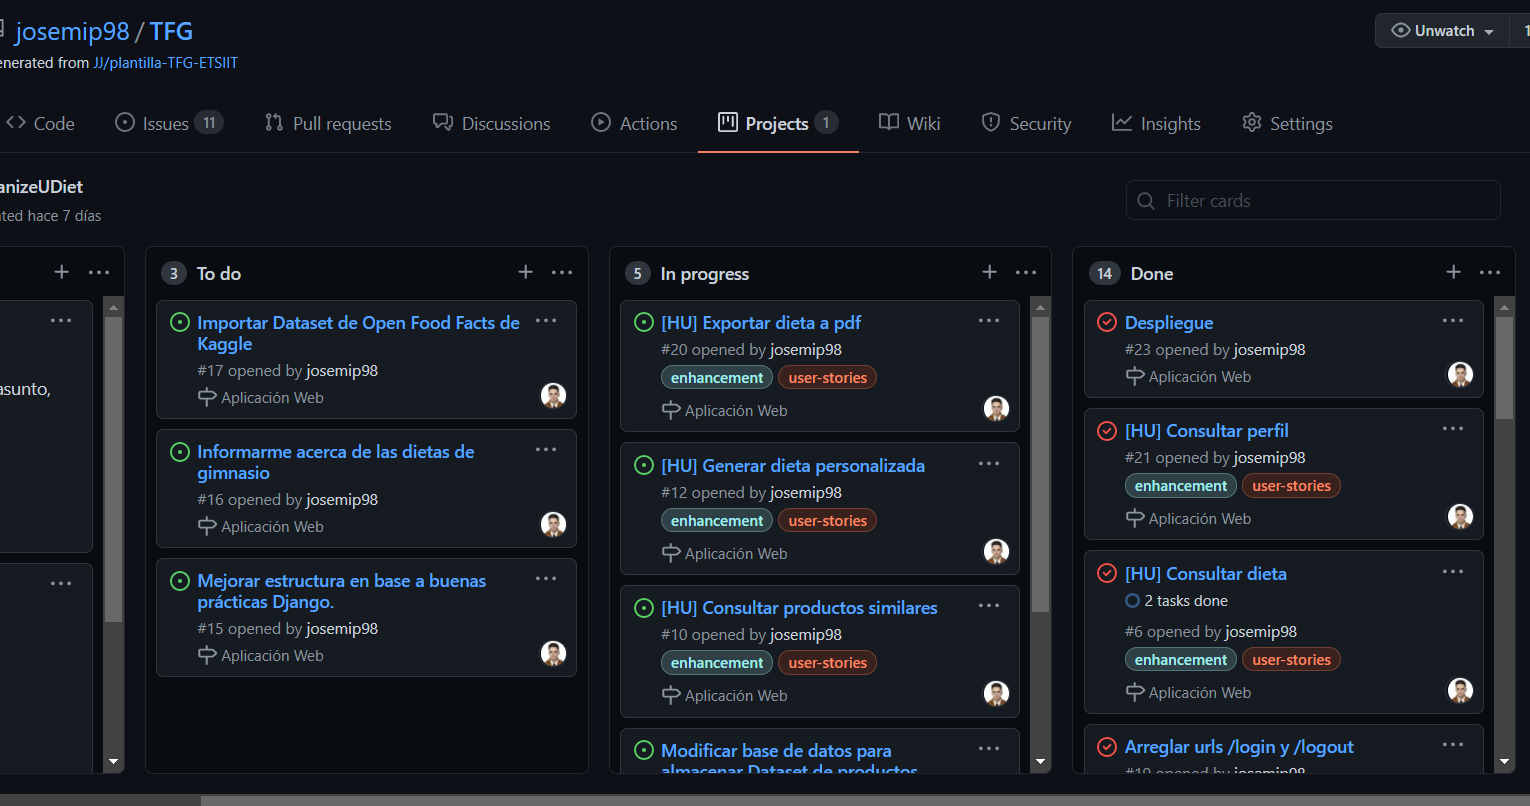
\includegraphics[scale=0.4]{kanban.png}}
  \caption{Tabla Kanban del proyecto.}
\end{figure}

\subsection{Hitos}

Los hitos o milestones se utilizan como agrupación de issues o pull requests englobando un grupo de problemas o problemas más grandes que resolver.
Por ejemplo yo para mi proyecto he creado un sólo milestone llamado aplicación web pero se podría crear otro que fuera aplicación móvil para en un futuro realizarla y en dichos hitos irían todas las issues relacionadas.

\begin{figure}[H]
	\centering
	\noindent\makebox[\textwidth]{
	  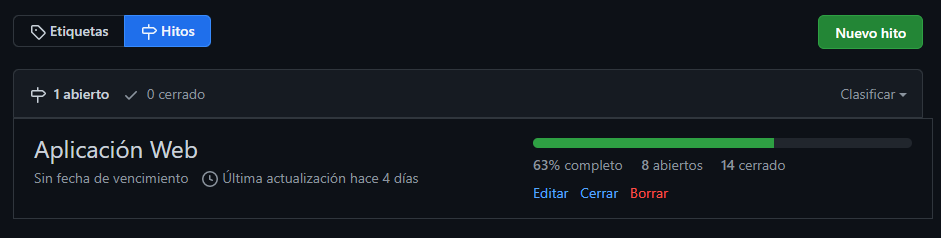
\includegraphics[scale=0.4]{hito.png}}
	\caption{Ejemplo épica del proyecto.}
  \end{figure}

\subsection{Historia de usuario}
Una historia de usuario es \textbf{una funcionalidad que el usuario espera}.
El modelo a seguir para la creación de historias de usuario es:

\textit{Como usuario/desarrollador quiero poder [funcionalidad] para [razón dicha funcionalidad].}

Además podemos añadir tareas que necesitamos cumplir para completar la historia de usuario o detalles técnicos.

\begin{figure}[H]
	\centering
	\noindent\makebox[\textwidth]{
	  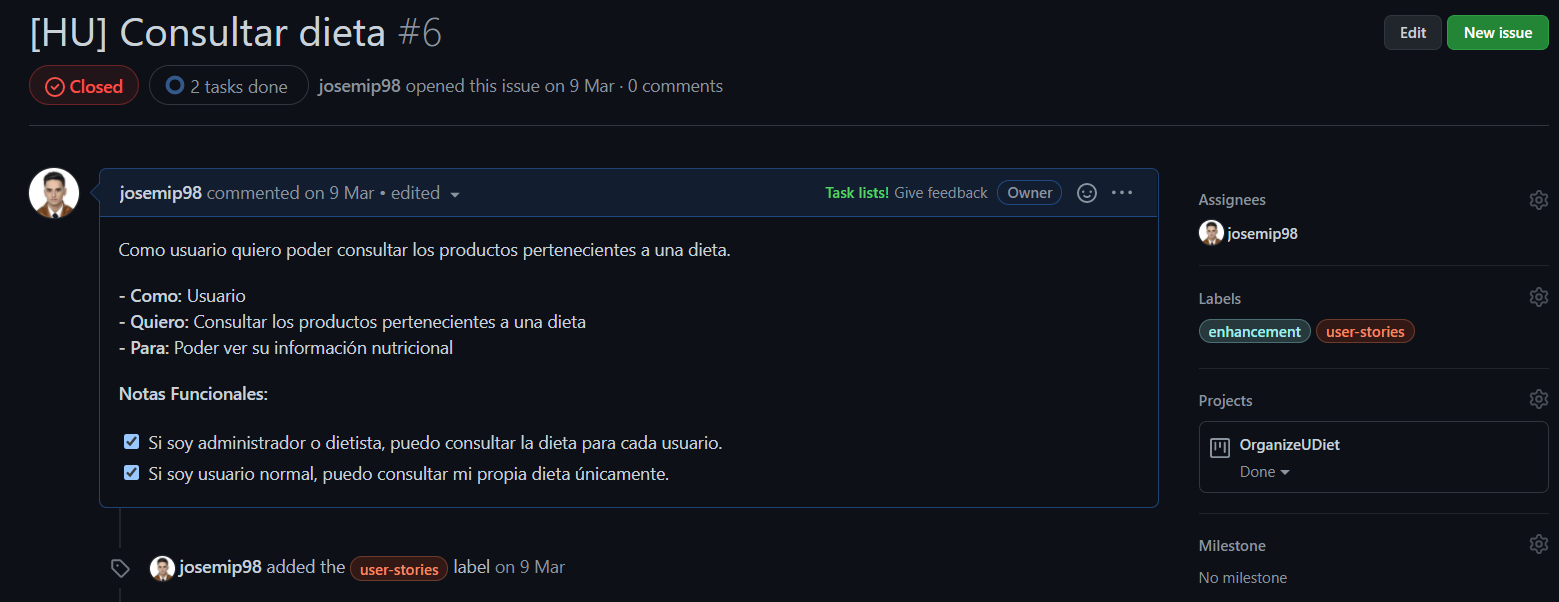
\includegraphics[scale=0.4]{hu.png}}
	\caption{Ejemplo historia de usuario.}
  \end{figure}

\subsection{Issues}
Las issues pueden ser correción de bugs, tareas que sean necesarias para el desarrollo o mantenimiento del proyecto.

\begin{figure}[H]
	\centering
	\noindent\makebox[\textwidth]{
	  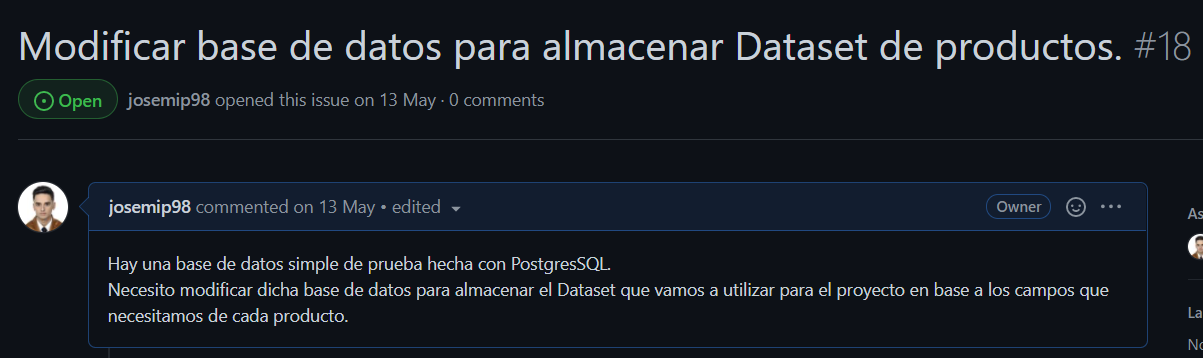
\includegraphics[scale=0.4]{issue.png}}
	\caption{Ejemplo de issue.}
  \end{figure}

\subsection{Etiquetas}

Las etiquetas son la forma de categorizar las issues pendientes ya sea asignandoles prioridad o describiendo si es una issue de documentación, si es un bug, historia de usuario...
Además podemos crear etiquetas a nuestro gusto según las necesidades que tengamos.

\begin{figure}[H]
	\centering
	\noindent\makebox[\textwidth]{
	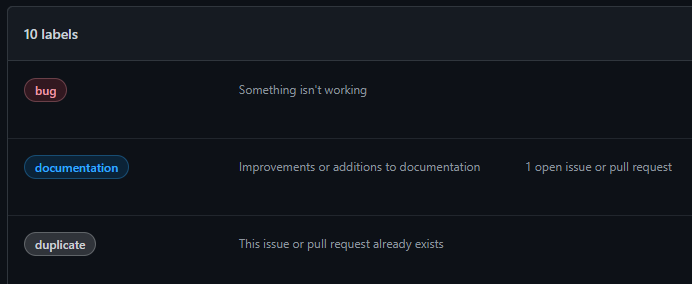
\includegraphics[scale=0.4]{etiquetas.png}}
	\caption{Ejemplo de etiquetas.}
\end{figure}

	% Implementación
	\chapter{Implementación} \label{sec:implementacion}

\section{Tecnologías empleadas} \label{sec:tecnologias}

En este apartado voy a indicar las necesidades del proyecto para así elegir que tecnologías vamos a utilizar, porqué las vamos a utilizar y que otras opciones teníamos.

\subsection{Framework}

Necesitamos un Framework para desarrollo web de los que podemos destacar \textbf{Django, Laravel y Express} como los más conocidos y utilizados.
Para elegir con cuál quedarnos voy a explicar cuáles son las necesidades del proyecto y las características de cada uno de estos Frameworks.\\\\
\\
Para el proyecto necesitamos un Framework que trabaje con bases de datos, que trabaje la programación orientada a objetos y que trabaje 
mediante el patrón MVC (Modelo-Vista-Controlador) para poder llevar a cabo un desarrollo ágil y reutilizable, que tenga flexibilidad, 
un gran entorno de librerías y buena comunidad.\\
\\\\
Una vez determinadas nuestras necesidades, vamos a explicar que nos pueden aportar los Frameworks mencionados anteriormente a conseguir satisfacer estas necesidades.\\\\

"\textbf{Django} es un framework web completo ampliamente usado. Cuenta con un motor de plantillas propio (muy similar a Jinja 2) así una arquitectura Modelo/Vista/Controlador" \cite{django}.
Está basado en \textbf{Python}, cuenta con un gran entorno de librerías tanto para sistema de autentificación de usuarios, manejo de imágenes, paginador, etc..., gran rendimiento, flexibilidad,
pero sobre todo que permite un desarrollo ágil y reutilizable siguiendo el modelo MVC.\\ \\

Otros Frameworks como Laravel, Laravel, Spring o Express utilizan tambien el modelo MVC y tienen características similares pero he decidio quedarme con \textbf{Django} porque es el que conozco de 
haberlo utilizado en el grado de ingeniería informática y me siento más cómodo trabajando con él.\\ \\

Django utiliza el modelo MVC, aunque en su caso es \textbf{MVT (Modelo-Vista-Template)}.\\
El \textbf{modelo} maneja las tablas de la base de datos, la validación y las consultas.\\
Las \textbf{vistas} serían las funciones que enlazan los modelos con los templates y deciden que template se muestra.\\
Los \textbf{templates} son la información que se muestra.\\ 

La diferencia con otros modelos MVC es la vista, que en este caso las vistas serían el controlador y los templates serían las vistas.
Por último, voy a explicar el funcionamiento de dicho modelo:

\begin{figure}[H]
  \centering
  \noindent\makebox[\textwidth]{
    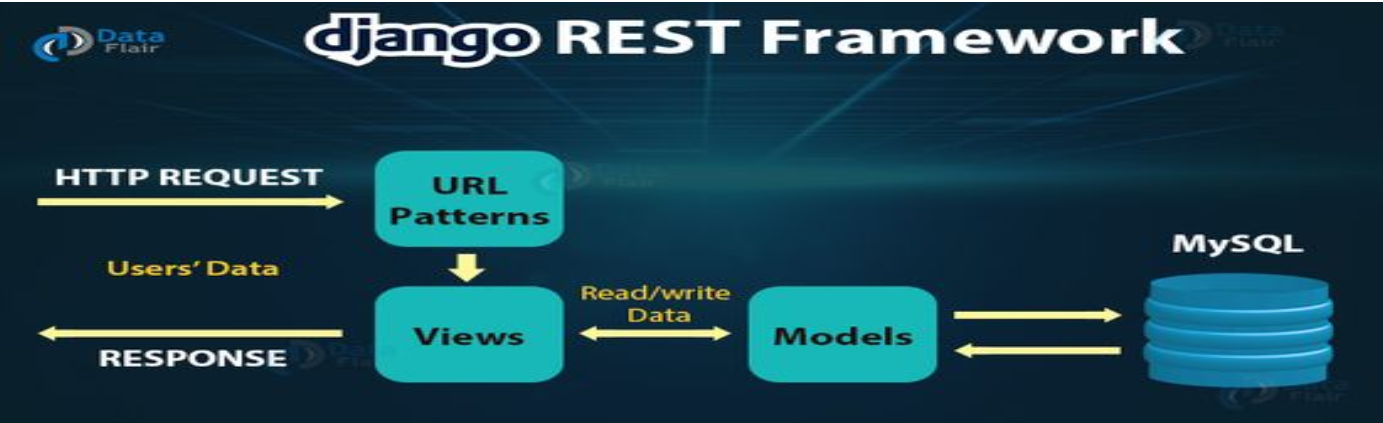
\includegraphics[scale=0.6]{django.png}}
  \caption{Modelo-Vista-Template Django}
\end{figure}

Cuando hacemos una consulta a la web, esta consulta accede al mapa de URLs, cada ruta está asociada a una vista, 
esa vista decide si necesita hacer una consulta a la base de datos, y, por tanto, irá a los modelos y después se 
mostrará la información a través de un template o directamente se muestra la información en un template.

\subsection{Lenguaje de programación}

Una vez elegido el Framework \textbf{Django}, como lenguaje de programación no nos queda otra que utilizar \textbf{Python} como lenguaje de programación.\\\\
\textbf{Python} es un lenguaje multipropósito, es entendible y simple, además de tener una curva de aprendizaje baja frente a otros lenguajes tan estrictos como \textbf{C}, 
tiene gran variedad de Frameworks, gran entorno de librerías y es multiplataforma.\\ \\

\section{Base de datos} \label{sec:base_datos}

\subsection{Tecnología}

Para elegir que gestor de base de datos utilizar en el proyecto primero debemos pensar en qué necesidades tenemos.
Las dos características principales que deben cumplir es que sea escalable y que funcione bien en ambientes de alto volumen 
de datos ya que la aplicación comenzará a funcionar con un número pequeño de productos alimenticios pero la idea es almacenar una gran cantidad de datos.\\ \\
Mis opciones eran \textbf{PostgreSQL} y \textbf{MongoDB}, aunque obviamente hay muchas más opciones, estas son las que conozco de haber trabajado con ellas y
más fácil me va a ser trabajar con ellas.\\ \\

En ese aspecto tanto \textbf{PostgreSQL} como \textbf{MongoDB} son buenas opciones ya que cumplen esas características.\\ \\

"\textbf{MongoDB} \cite{NoSQL} es una base de datos NoSQL potente que nos permitirá almacenar cualquier información que nuestra aplicación web necesite. Desde Python podemos acceder a la base de datos MongoDB usando el cliente Pymongo".

Por otro lado, \textbf{PostgreSQL} es una base de datos SQL también muy potente, con gran escalabilidad y con la que podremos almacenar cualquier información que necesitemos.\\

Ambas son muy buenas opciones para nuestro proyecto pero finalmente me he decidido por \textbf{PostgreSQL}, ya que para el despliegue \ref*{sec:despliegue} nos va a facilitar mucho las cosas
al tener un uso gratuito con \textbf{Heroku}.

\subsection{Configuración}

Una vez creado nuestro proyecto de Django, por defecto nos viene configurado para usar sqlite, pero configurarlo con PostgreSQL va a ser muy sencillo.
Simplemente tenemos que instalar la librería \textbf{psycopg2} y en el archivo settings crear una base de datos que tenga el motor de PostgreSQL en lugar de sqlite3.
Además, debemos indicarle un nombre, host, credenciales de usuario y contraseña y puerto (normalmente 5432).\\ \\

Una vez hecho esto debemos crear nuestros modelos de la base de datos.

\subsection{Modelos}

Para el diseño de las estructuras de datos y en este caso, los modelos, se va a seguir el \textbf{diseño guiado por el dominio} \cite{DDD} (domain-driven design o DDD).\\ \\

Es un serie de prácticas y terminologías que hacen que se cree una comunicación efectiva entre expertos del dominio, en este caso dietistas, nutricionistas o gente con 
grandes conocimientos acerca de la alimentación, y los desarrolladores.\\

\begin{figure}[H]
  \centering
  \noindent\makebox[\textwidth]{
    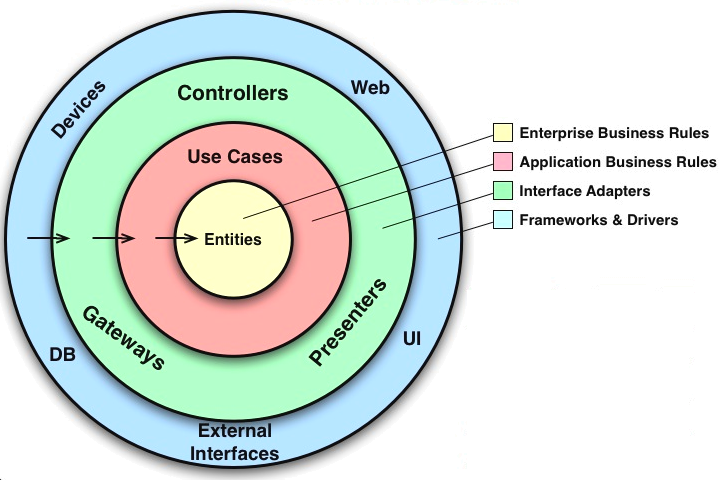
\includegraphics[scale=0.5]{domain-driven-design.png}}
  \caption{Domain-Driven-Design}
\end{figure}

Como se muestra en la figura, tenemos en el centro de todo las entidades o modelos. Una vez creados estos modelos, serán los propios usuarios y expertos en el modelo de negocio los que
mediante historias de usuario van a detallar las distintas funcionalidades que tendra el proyecto. A partir de ahí se crean los controladores (backend) y por último, tenemos el frontend,
en nuestro caso, una web.\\ \\

Esta manera de diseño hace que las capas más internas no sepan nada acerca de las externas, mientras que las externas se basan en las internas.

He creado los modelos producto, dieta y usuario, los modelos E/R se encuentran en el apéndice \ref*{apendiceB}\\
El modelo producto está formado por 23 datos que guardan información del producto como nombre, tienda, categoría.. y información nutricional como proteinas, hidratos, grasa...\\\\

\begin{figure}[H]
  \centering
  \noindent\makebox[\textwidth]{
    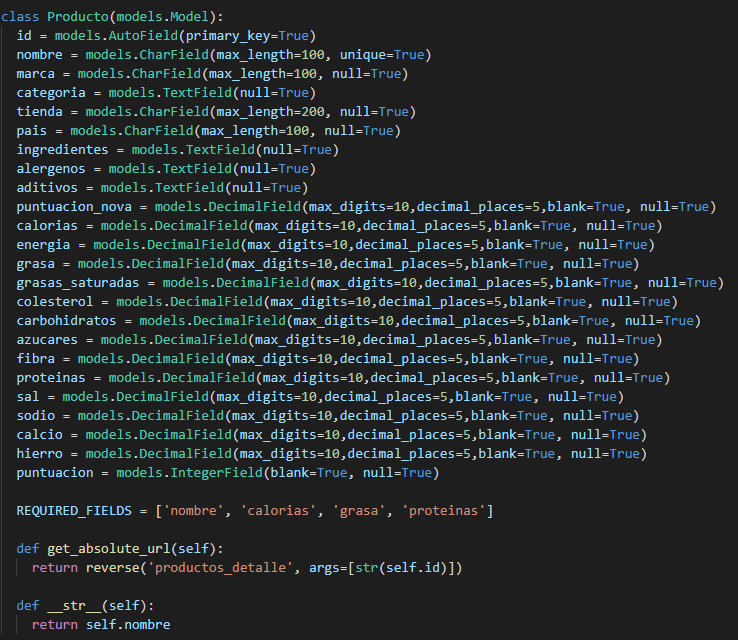
\includegraphics[scale=0.7]{productoModel.png}}
  \caption{Modelo producto}
\end{figure}

El modelo dieta está formado por un nombre, una descripción, una lista de productos y un usuario al que se le asigna.\\

\begin{figure}[H]
  \centering
  \noindent\makebox[\textwidth]{
    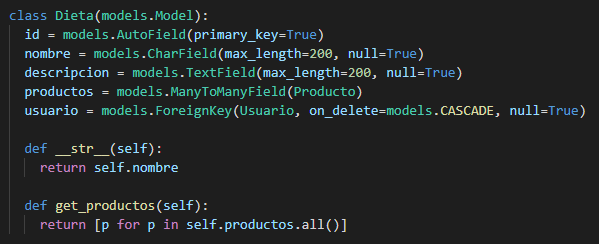
\includegraphics[scale=0.7]{dietaModel.png}}
  \caption{Modelo dieta}
\end{figure}

Para el modelo del usuario he utilizado la librería \textbf{django.contrib.auth.models} de Django, 
esta librería nos da toda la funcionalidad necesaria para crear usuarios, iniciar sesión y cerrarla. 
El problema es que sólo tiene los atributos username, password, email, nombre y apellidos.\\\\

Para solucionar esto he utilizado otra librería llamada \textbf{Base Abstract user} que te permite a partir 
de la librería anterior crear un modelo de usuario modificado con los atributos que nosotros queramos.\\

Para ello creamos el siguiente modelo de usuario, en el que tenemos atributos como peso, altura, edad, sexo y fecha de nacimiento.

\begin{figure}[H]
  \centering
  \noindent\makebox[\textwidth]{
    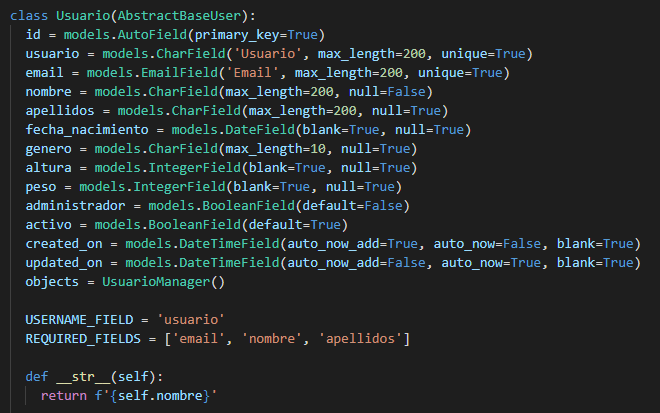
\includegraphics[scale=0.7]{usuarioModel.png}}
  \caption{Modelo usuario}
\end{figure}

Una vez tenemos el modelo de usuario simplemente en el settings indicamos dicho modelo y creamos las funciones 
para crear usuarios y súper usuarios.\\

\begin{figure}[H]
  \centering
  \noindent\makebox[\textwidth]{
    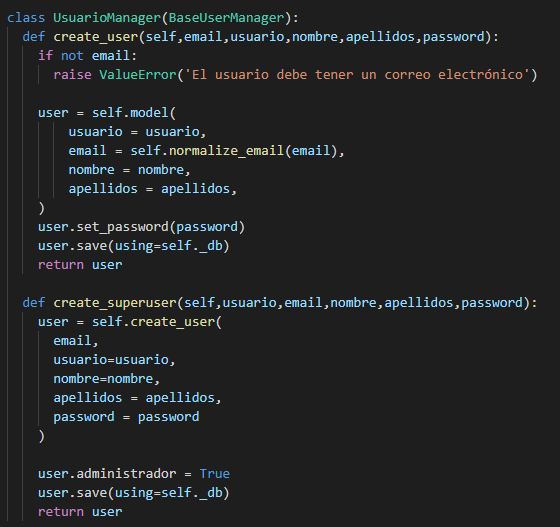
\includegraphics[scale=0.7]{usuarioManager.png}}
  \caption{Modelo usuario manager}
\end{figure}

\subsection{Datos}

Los datos han sido descargados de la web de \textbf{Open Food Facts}, como expliqué en la sección de estado del arte \ref{sec:estado_del_arte}.
Han sido utilizados porque es una gran cantidad de productos los que contiene esa base de datos y te permite descargarlos en diferentes formatos y, muy importante,
son de código abierto.\\ \\

En esta ocasión he obtenido los datos en formato CSV y para la limpieza de datos he utilizado \textbf{Excel}, sin embargo, la idea es automatizar esta tarea en un futuro
con \textbf{scripts de Python}, para ello podriamos utilizar la librería \textbf{Pandas}.

En cuanto a eliminar campos he hecho lo siguiente:
\begin{enumerate}
  \item He eliminado los productos cuyo nombre estuviera vacío.
  \item He eliminado valores que no fueran correctos:
  \begin{itemize}
    \item Valores calóricos que eran exageradamente grandes.
    \item Valores calóricos que eran exageradamente pequeños.
  \end{itemize}
  \item Campos que contenían caracteres especiales
\end{enumerate}

Una vez eliminados esos valores, he filtrado por productos que son procedentes de España ya que por el momento me eran suficientes.
Cuando el proyecto vaya avanzando en el desarrollo se irán incluyendo productos de otros países, pero ahora mismo la base de datos era
 demasiado grande para las herramientas que he utilizado en el despliegue \ref{sec:despliegue}.\\

\section{Backend} \label{sec:backend}

Voy a explicar la funcionalidad de la aplicación, así como las funciones más interesantes y las bibliotecas o paquetes utilizados para ello, podemos consultar el manual de usuario en el apéndice C \ref*{apendiceC}. \\ \\

Para el modelo de usuario podemos registrarnos y crear nuestro perfil, a demás de consultarlo, modificarlo y eliminarlo.
Si iniciamos sesión podemos consultar el lsitado total de productos que hay en la web así como buscar el que queramos, consultarlo en detalle y
modificarlo y eliminarlo si somos administradores o pertenecemos al grupo de dietistas.\\ \\

Para el paginador de la vista listado de productos he utilizado \textbf{django.core.paginator} de Django. Este paquete nos permite crear 
un paginador muy fácil simplemente llamamos a la función Paginador pasándole dos parámetros, un listado con los objetos que 
queramos mostrar y el número en el que queremos dividirlo (productos a mostrar por página). \\ \\

Para la generación de dietas en un principio la idea era utilizar un algoritmo de la mochila con el que a partir de un formulario obtuvieramos los datos del solicitante
como el peso, altura, sexo y objetivos, y en base a eso obtener unas cantidades de proteinas, grasas, etc que tuvieramos que alcanzar.\\ \\

El algoritmo trabajaría con esos parámetros y generaría una dieta que alcanzara esas cantidades de nutrientes específicos, pero finalmente esa idea fué descartada por dos motivos.\\\\

Primero por eficiencia, ya que queremos tener una gran cantidad de productos y un algoritmo así tardaría una gran cantidad de tiempo en hacer esos cálculos, además el otro motivo es 
porque la gente con conocimientos sobre nutrición, como dietistas y culturistas, a la que he consultado me han comentado lo mismo, que no se puede conseguir una dieta optimizada con esos 
parámetros ya que es todo mucho más complicado, es decir, de esa manera obtendriamos una dieta optimizada con la que ganar peso para una persona y esa misma dieta para otra persona con 
las mismas características no obtendrían los mismos resultados. Esto es debido a nuestros metabolismos y es muy complicado calcularlo.\\\\

Ante esto, entre yo y estas personas pensamos que lo mejor era poder solicitar estas dietas pero que en vez de generarlas con un algoritmo de la mochila, estuvieran ya creadas previamente
y sólo se tendría que elegir una en función de los objetivos y características del usuario. Una vez obtenida la dieta, para optimizarla vamos a desarrollar una función con la que 
obtengamos productos que sean similares entre sí, nutricionalmente hablando.\\\\

Esto haría que nosotros podamos ir probando nuevos productos e incluirlos en nuestras dietas en función de qué nos va mejor o peor, además nos da la opción de encontrar productos más asequibles de precio si así los quisieramos y que se ajustaran más a nuestros gustos.

\section{Frontend} \label{sec:frontend}

Para el Frontend del proyecto a desarrollar vamos a realizar una \textbf{aplicación web} ya que para los dietistas les va a ser mucho más cómodo
crear sus dietas y consultar información que, desde una aplicación móvil, y para los demás usuarios pueden consultarlo desde otros dispositivos, si así lo quisieran, 
debido a que el diseño va a ser adaptable para todo tipo de dispositivos.

Para ello, voy a utilizar \textbf{Bootstrap} \cite{bootstrap} ya que nos permite diseñar sitios webs de manera sencilla,
es de código abierto, es compatible con todos los navegadores y sus diseños son adaptables por lo que funcionan en todos los dispositivos,
además, es muy completo y presenta una gran variedad de componentes muy útiles como modales, tablas, alertas, botones...\\ \\

La idea de diseño de la web ha sido cogida de la plantilla de \textbf{AdminLTE} \cite{adminlte}. Esta plantilla es de código abierto y 
además, incluye muchos componentes útiles.

Para los iconos he utilizado la web open source \textbf{FontAwesome} \cite{iconos} que nos 
ofrece una gran cantidad de iconos gratis además de dar la capacidad de elegir el tamaño de ellos.

\subsection{Formularios}

Otra parte importante serán los formularios, con estos podremos crear y modificar los modelos creados anteriormente.

\begin{figure}[H]
  \centering
  \noindent\makebox[\textwidth]{
    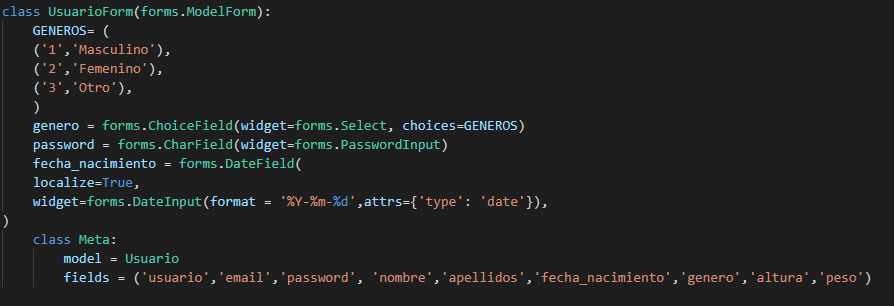
\includegraphics[scale=0.7]{usuarioForm.png}}
  \caption{Formulario de usuario}
\end{figure}

\begin{figure}[H]
  \centering
  \noindent\makebox[\textwidth]{
    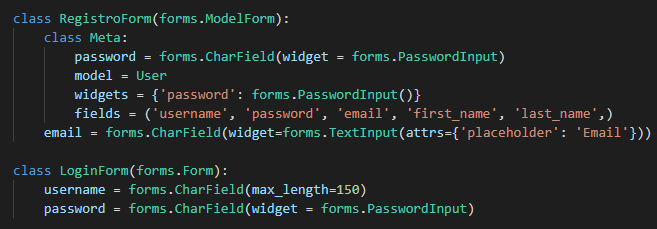
\includegraphics[scale=0.7]{registroLoginForm.png}}
  \caption{Formularios de registro y login}
\end{figure}

\newpage
\section{Tests} \label{sec:tests}

Los tests son una parte muy importante del proyecto ya que sin ellos no sabes si has llevado a cabo las historias de usuario o no, por tanto, 
podemos decir que es la forma de asegurar la calidad del software. \\ \\

Para los tests emplearé la biblioteca \textbf{TestCase}. Es la más común en Django para la creación de test.\\
Esta biblioteca es una extensión de SimpleTestCase, pero esta sólo vale si no utilizas una base de datos 
en tu aplicación.\\

Para cada una de las funcionalidades de la web vamos a crear un test y con ella cerraremos la issue corespondiente.
Este sería un ejemplo en la que testeamos las funciones de crear y modificar un producto.

\begin{figure}[H]
  \centering
  \noindent\makebox[\textwidth]{
    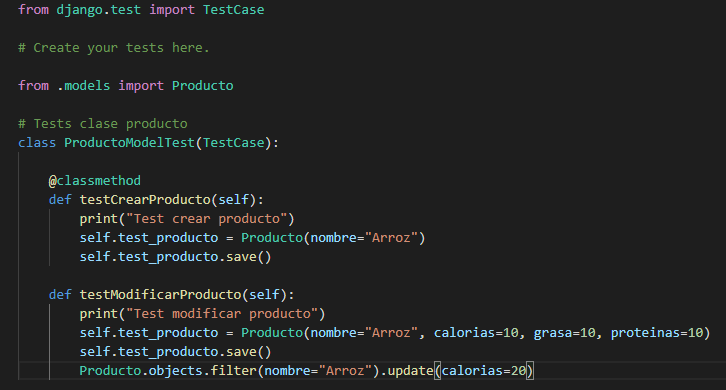
\includegraphics[scale=0.7]{test.png}}
  \caption{Test}
\end{figure}

\section{Despliegue} \label{sec:despliegue}

\subsection{Plataforma}

Por último, quedaría desplegar la aplicación, para ello voy a utilizar \textbf{Heroku}.\\

Ante las necesidades del proyecto de encontrar una plataforma de despliegue en la nube que fuera fácil de usar, pudiera actualizarse de manera automática, fuera gratuita y permitiese el lenguaje Python decidí utilizar Heroku ya que cumplía todas estas necesidades. 

\textbf{Heroku} es una plataforma en la nube que nos permite desplegar aplicaciones web en cualquier lenguaje de programación.
Además, es muy sencillo, sólo tenemos que conectar nuestro repositorio de GitHub en el que tengamos el proyecto que queremos desplegar,
podemos configurarlo para que con cada commit se haga el despliegue automáticamente y además es gratuito. Otras alternativas a Heroku 
eran Firebase y Azure.

\subsection{Librerías}

La primera librería que tenemos que instalar es \textbf{Gunicorn}. Esta librería es un servidor HTTP para Unix, sin ella nos sería imposible realizar el despliegue de nuestra aplicación.
Como en este proyecto estamos trabajando con base de datos PostgreSQL, necesitamos instalar la librería \textbf{psycopg2}. Esta librería es un adaptador a dicha base de datos para el lenguaje Python.\\\\
Heroku por defecto no permite los archivos estáticos, para solucionar este problema he incluido la librería \textbf{whitenoise}.\\
Esta librería nos permite cargar todos los archivos estáticos y se configura muy fácil, simplemente tenemos que instalarlo y en
el fichero settings.py de la aplicación incluimos el middleware y las rutas de dichos archivos que queremos cargar.\\\\
Por último, necesitamos dos librerías más, una de ellas es \textbf{dj-database-url}. Esta librería realiza la conexión entre nuestro proyecto y el gestor de base de datos de Heroku.\\
Y la otra librería es \textbf{python-decouple} para usar variables de entorno en Heroku, así evitamos poner tokens y contraseñas a la vista de todos en nuestro proyecto. \\

Por tanto, el archivo requirements.txt quedaría así:
\begin{figure}[H]
  \centering
  \noindent\makebox[\textwidth]{
    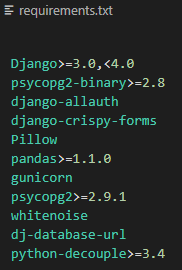
\includegraphics[scale=1]{requirements.png}}
  \caption{Archivo requirements.txt}
\end{figure}


\subsection{Configuración}

Para configurar el despliegue en Heroku como he explicado anteriormente debemos registrarnos en la web y conectar el repositorio de Github del proyecto.
Una vez hecho esto nos vamos al archivo settings.py del proyecto y hacemos lo siguiente:\\
Importamos las librerías, ponemos debug a false e incluimos en allowed\_hosts la url de despliegue o simplemente ponemos un asterisco y así acepta todas las urls.

\begin{figure}[H]
  \centering
  \noindent\makebox[\textwidth]{
    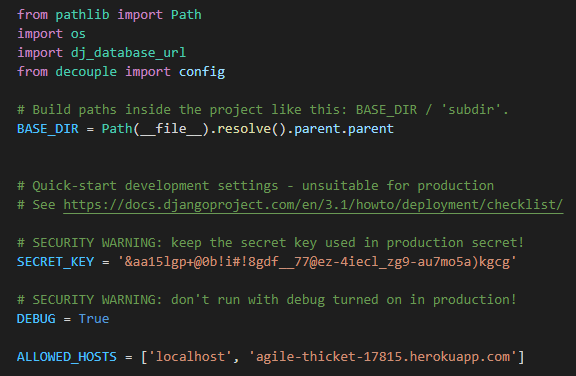
\includegraphics[scale=0.8]{settings1.png}}
  \caption{Configuración despliegue}
\end{figure}

Añadimos el middleware de whitenoise.

\begin{figure}[H]
  \centering
  \noindent\makebox[\textwidth]{
    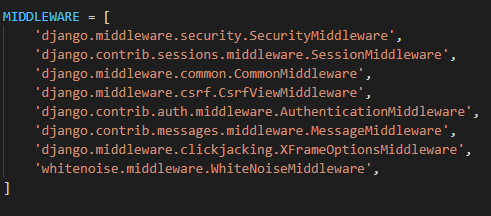
\includegraphics[scale=1]{settings2.png}}
  \caption{Configuración despliegue middleware}
\end{figure}

Indicamos la base de datos.

\begin{figure}[H]
  \centering
  \noindent\makebox[\textwidth]{
    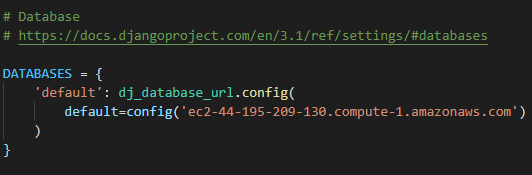
\includegraphics[scale=1]{settings3.png}}
  \caption{Configuración despliegue base de datos}
\end{figure}

Añadimos esta línea para que whitenoise cargue los archivos estáticos.

\begin{figure}[H]
  \centering
  \noindent\makebox[\textwidth]{
    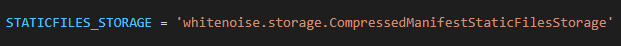
\includegraphics[scale=1]{settings4.png}}
  \caption{Configuración despliegue archivos estáticos}
\end{figure}

Ya tendríamos configurado todo. Simplemente tenemos que esperar a que se haga el despliegue si hemos configurado que se haga automáticamente con cada commit o desplegarlo nosotros desde la web.\\\\

Otra opción sería hacerlo desde local.
Nos conectamos a nuestra cuenta de Heroku con Heroku login, creamos una app de heroku con heroku create y hacemos un push desde nuestro repositorio local con:
\begin{lstlisting}
git push --prefix app keroku master
\end{lstlisting}

Conectamos nuestra base de datos con nuestra app con el siguiente comando:
\begin{lstlisting}
heroku pg:psql <nombre_bd_heroku> --app <nombre_app_heroku>
\end{lstlisting}

Ahora sólo quedaría hacer un migrate de la base de datos con:
\begin{lstlisting}
heroku run python manage.py migrate
\end{lstlisting}

Incluimos nuestros archivos sql con nuestros datos de la base de datos.
\begin{lstlisting}
heroku pg:psql --app <nombre_app> < <archivo.sql>
\end{lstlisting}
Y abrimos la aplicación con heroku open.\\\\

Para probar la aplicación aquí dejo el enlace:

\url{https://organize-udiet.herokuapp.com/}

\section{Presupuesto} \label{sec:coste}

\subsection{Planificación de costes}

En este apartado se va a realizar una estimación de costes del proyecto, ya que en todo proyecto de ingeniería los costes tanto de implementación como de ejecución son muy importantes.\\

Los factores a tener en cuenta para esta estimación van a ser:

\begin{enumerate}
  \item Duración del proyecto
  \item Sueldo del programador
  \item Plataforma de despliegue
\end{enumerate}

La duración del proyecto ha sido de unos 6 meses.\\

El sueldo medio de un programador \cite{sueldo} de mis carácteristicas (recien terminado el Grado de Ingeniería Informática y sin especializar en un lenguaje concreto) es de unos \textbf{20000\euro}.\\
Esto se traduce en unos \textbf{55\euro} al día, que trabajando a jornada de 8 horas serían unos \textbf{6,8\euro} la hora.\\

Por tanto, de los 210 días (7 meses) que ha durado el proyecto, a unas 3 horas de media trabajadas cada día serían 630 horas, que multiplicadas por el sueldo anteriormente mencionado sería un total de \textbf{4284\euro}.

En principio este sería el coste de desarrollo, a partir de ahí tenemos que pagar la plataforma de despliegue.\\ \\
Si elegimos \textbf{Azure} \cite{azure} que es una de las plataformas más utilizadas, un servidor con 4 núcleos, 7GB de RAM y 1000GB de almacenamiento nos costará \textbf{200\euro} cada mes que queramos tener la aplicación desplegada.\\


	% Conclusiones
	% Trabajos futuros
	\chapter{Conclusiones y trabajos futuros}

Este proyecto me ha permitido aprender mucho como programador web en muchos ámbitos desde
la planificación con GitHub mediante épicas, historias de usuario e issues que es como se 
trabaja en las empresas, las tecnologías actuales de desarrollo web como Python, Django, 
Postgres, Bootstrap, HTML, CSS y algunas más, que son las tecnologías que he utilizado en 
este proyecto además de las tecnologías probadas antes de la elección de las mencionadas 
anteriormente como por ejemplo Kotlin para el desarrollo de aplicaciones móviles, ángular, 
react, php, laravel, etc.
\\\\
Sobre el proyecto, era un tema que me interesaba bastante por lo que me ha sido más fácil 
trabajar sobre ello y me gustaría continuarlo en un futuro añadiendo más funcionalidad a 
la aplicación web como pudiera ser un calendario para organizar las comidas diarias, mejorar 
los algoritmos de creación de dietas y de similitud de alimentos mediante investigación 
nutricional, expansión de la base de datos de productos, capacidad de hacer un seguimiento
sobre el usuario en términos de peso, grasa, músculo, etc.. e incluso meterme en temas de 
ejercicios y planes de gimnasio para así ya tener todo lo que necesitas para estar saludable 
y en forma. Todo eso y más ideas que puedan ir surgiendo.
\\\\
Por tanto, puedo decir que estoy muy contento con todo el aprendizaje que he tenido realizando 
el proyecto, ya que me ha desarrollado como programador web y me siento orgulloso por ello ya 
que me ha ayudado a la hora de encontrar trabajo y conseguir experiencia laboral en este tema 
que tanto me interesa.

	
	\newpage
	\bibliography{bibliografia}
	\bibliographystyle{plain}

	\appendix
	%\input{secciones/personas.tex}
	\chapter{Historias de usuario}

En este apartado se muestran las distintas historias de usuario que conforma toda la funcionalidad del proyecto.

\begin{enumerate}
	\item Registro \url{https://github.com/josemip98/TFG/issues/4}
    \item Login \url{https://github.com/josemip98/TFG/issues/5}
    \item Consultar productos \url{https://github.com/josemip98/TFG/issues/2}
    \item Consultar producto concreto \url{https://github.com/josemip98/TFG/issues/3}
    \item Consultar productos similares \url{https://github.com/josemip98/TFG/issues/10}
    \item Añadir un producto \url{https://github.com/josemip98/TFG/issues/7}
    \item Modificar un producto \url{https://github.com/josemip98/TFG/issues/8}
    \item Eliminar un producto \url{https://github.com/josemip98/TFG/issues/9}
    \item Editar perfil \url{https://github.com/josemip98/TFG/issues/11}
    \item Consultar perfil \url{https://github.com/josemip98/TFG/issues/21}
    \item Generar dieta personalizada \url{https://github.com/josemip98/TFG/issues/12}
    \item Consultar dieta \url{https://github.com/josemip98/TFG/issues/6}
    \item Exportar dieta a pdf \url{https://github.com/josemip98/TFG/issues/20}
    \item Apariencia \url{https://github.com/josemip98/TFG/issues/13}
    \item Contenedor \url{https://github.com/josemip98/TFG/issues/14}
\end{enumerate}


	\chapter{Diagramas E/R}

En este primer apartado del apéndice se muestran los diagramas de entidad relación de las tablas Dieta, Producto y Usuario utilizadas 
para el desarrollo del proyecto.

\begin{figure}[H]
	\centering
	\noindent\makebox[\textwidth]{
	  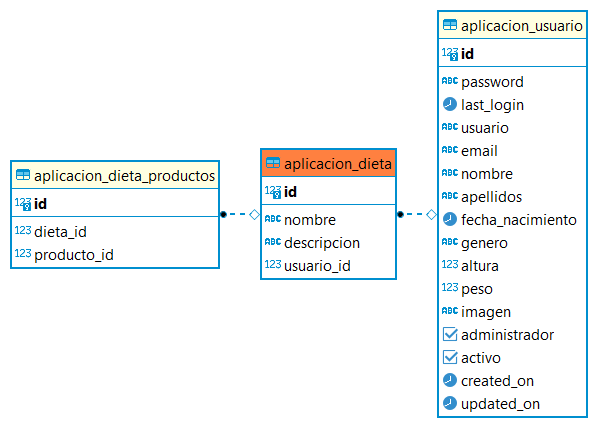
\includegraphics[scale=0.4]{aplicacion_dieta.png}}
	\caption{Diagrama para tabla de dietas.}
\end{figure}

\begin{figure}[H]
	\centering
	\noindent\makebox[\textwidth]{
	  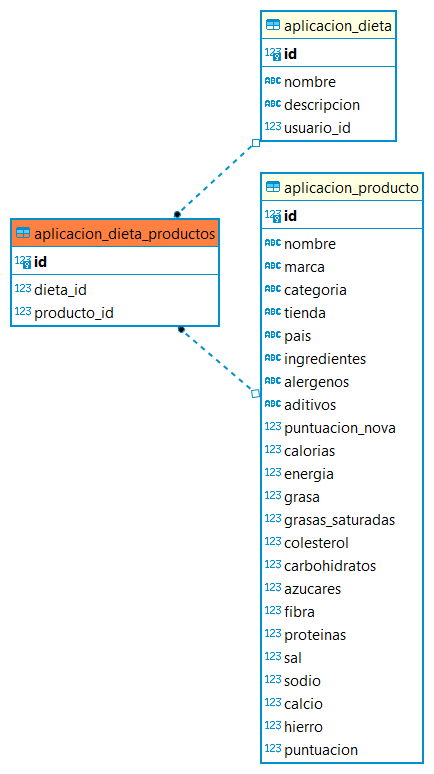
\includegraphics[scale=0.4]{aplicacion_dieta_productos.png}}
	\caption{Diagrama para tabla relación dietas y productos.}
\end{figure}

\begin{figure}[H]
	\centering
	\noindent\makebox[\textwidth]{
	  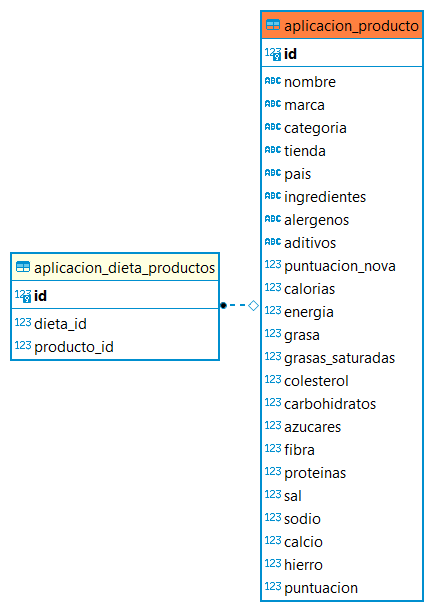
\includegraphics[scale=0.4]{aplicacion_producto.png}}
	\caption{Diagrama para tabla de productos.}
\end{figure}

\begin{figure}[H]
	\centering
	\noindent\makebox[\textwidth]{
	  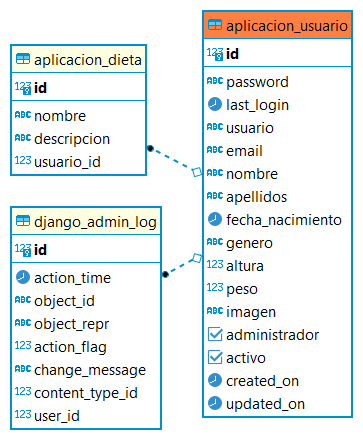
\includegraphics[scale=0.4]{aplicacion_usuario.png}}
	\caption{Diagrama para tabla de usuarios.}
\end{figure}
	
\end{document}

